\documentclass[a4paper]{article}

\def\ssver{4.0.81}

\usepackage[left=1cm,right=1cm,top=0.75cm,bottom=2cm]{geometry}
\usepackage{xcolor}
\usepackage{pdfpages}
\usepackage{fancyhdr}
\usepackage[hyperindex]{hyperref}
\usepackage{makeidx}
\usepackage{graphicx}
\usepackage{adjustbox}
\usepackage{multicol}
\usepackage{totcount}
\usepackage{xcolor}

% Index
\makeindex

% Counters
\newtotcounter{songcount}
\newtotcounter{psalmcount}
\definecolor{title dark}{HTML}{7E73A7}

% Footer
\pagestyle{fancy}
\fancyhf{}
\cfoot{{\small\thepage} \\ v{\ssver}}
\renewcommand{\headrulewidth}{0pt}

\makeatletter

% Chorus
\newcommand{\chorus}{\@chorusi}
\newcommand{\@chorusi}{\@ifnextchar\end{\@chorusend}{\@chorusii}}
\newcommand{\@chorusii}[1]{\quad{\itshape#1}\par\@chorusi}
\newcommand{\@chorusend}[1]{\vskip1em}

% --------------------

% Verse
\renewcommand{\verse}{\@versei}
\newcommand{\@versei}{\@ifnextchar\end{\@verseend}{\@verseii}}
\newcommand{\@verseii}[1]{#1\par\@versei}
\newcommand{\@verseend}[1]{\vskip1em}

% --------------------

% Bridge
\newcommand{\bridge}{\@bridgei}
\newcommand{\@bridgei}{\@ifnextchar\end{\@bridgeend}{\@bridgeii}}
\newcommand{\@bridgeii}[1]{{\itshape#1}\par\@bridgei}
\newcommand{\@bridgeend}[1]{\vskip1em}

\makeatother

% --------------------

% Songs
\newenvironment{song}[1]%
{%
    \begin{minipage}[t]{0.94\columnwidth}{\stepcounter{songcount}\textbf{\large #1}\index{#1}}%
        \par\vspace{2pt}
}%
{%
    \end{minipage}%
    \vspace{2em}%
}

\newenvironment{psalm}[2]%
{%
    \begin{minipage}[t]{0.94\columnwidth}%
        \begin{center}{\stepcounter{psalmcount}\textbf{\large #1}\index{#1}{\normalsize #2}}%
            \par\vspace{2pt}
}%
{%
    \end{center}%
    \end{minipage}%
    \vspace{2em}%
}%

\newcommand{\extra}[1]{{\normalsize\itshape (#1)}}

\renewcommand{\sp}{{\normalsize\itshape (Sing Psalms)}}
\newcommand{\tr}{{\normalsize\itshape (Scottish Psalter)}}
\newcommand{\LORD}{{\scshape Lord}}

\newcommand{\cp}[1]{{\tiny\ttfamily#1}}

% Chords
\definecolor{chordColor}{HTML}{CC241D}
\newcommand{\m}[2][l]%
{%
    \makebox[0pt][#1]%
    {%
      \begin{tabular}[b]%
        {@{}l@{}}%
        {\normalsize\mdseries\color{chordColor}#2}%
        \\%
        \mbox{}%
      \end{tabular}%
    }%
}

% Settings


\begin{document}
\sffamily
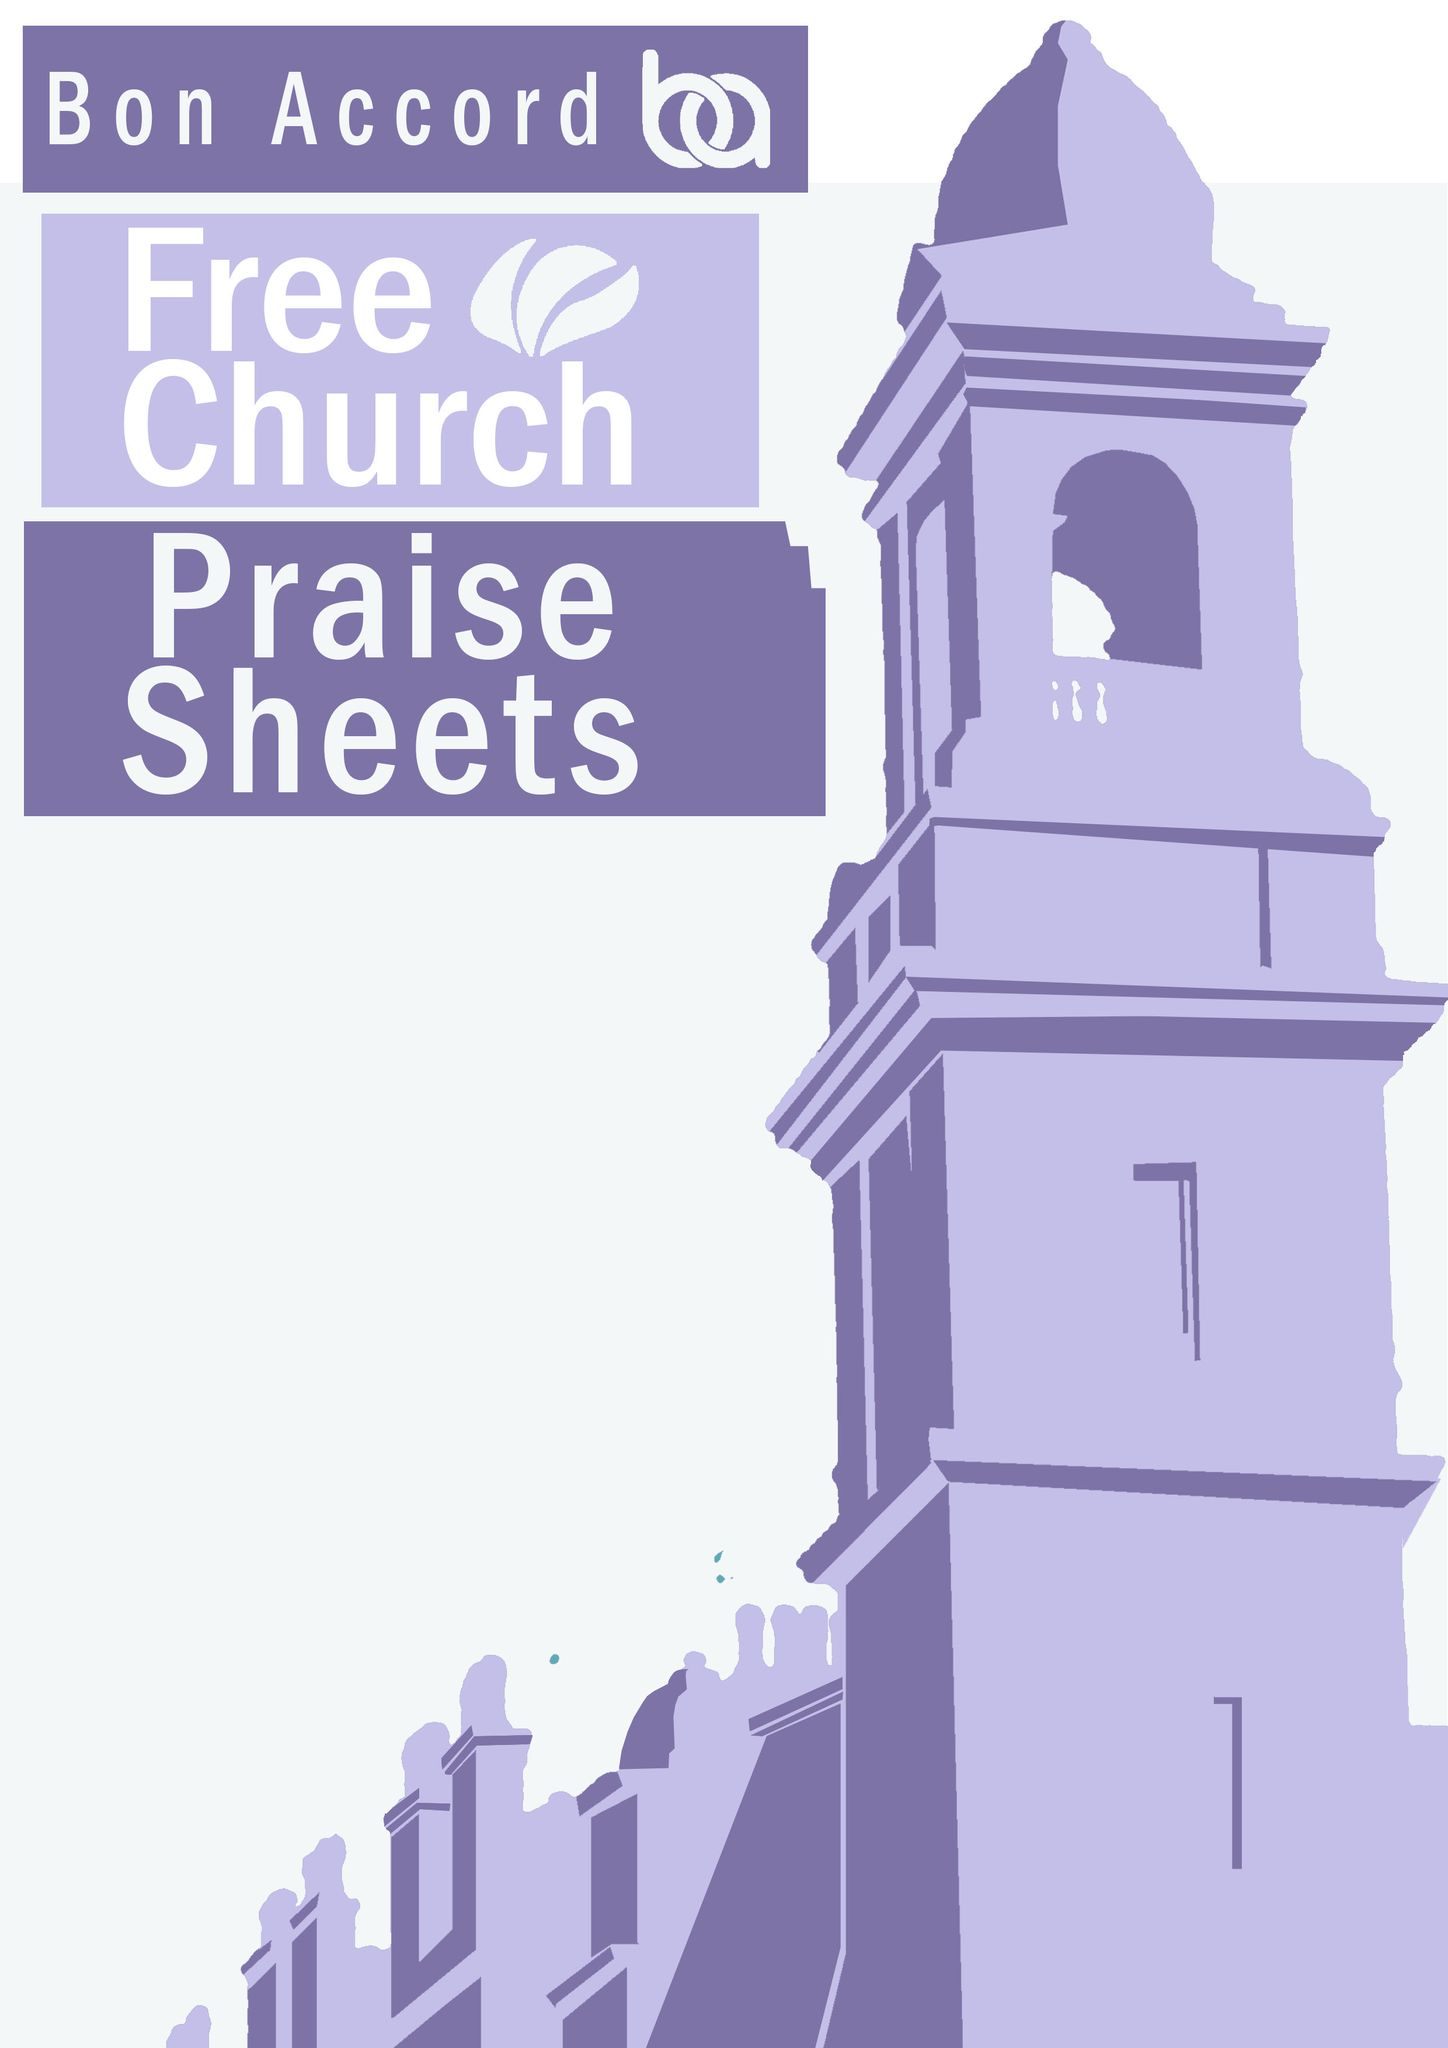
\includepdf{titleimage.jpg}
\setcounter{page}{2}  % Make title page, page 1
\printindex

% --------------------
\begin{multicols}{2}
\raggedcolumns

\begin{song}{Because He Lives}
    \verse
    {God sent His Son, they called him Jesus}
    {He came to love, heal and forgive}
    {He bled and died to buy my pardon}
    {An empty grave is there to prove my Saviour lives}
    \end
    \chorus
    {Because He lives, I can face tomorrow}
    {Because He lives all fear is gone}
    {Because I know He holds the future}
    {My life is worth the living just because He lives}
    \end
    \verse
    {How sweet to hold a new born baby}
    {And feel the pride and joy He gives}
    {But better still, the calm assurance}
    {That child can face uncertain days because He lives}
    \end
    \verse
    {And then one day I'll cross the river}
    {I'll fight life's final war with pain}
    {And then as death gives way to victory}
    {I'll see the lights of glory and I'll know He lives}
    \end
\end{song}

% ---

\begin{song}{As The Deer Pants}
    \verse
    {As the deer pants for the water}
    {So my soul longs after Thee.}
    {You alone are my heart's desire}
    {And I long to worship You}
    \end
    \chorus
    {You alone are my Strength, my Shield}
    {To You alone may my spirit yield}
    {You alone are my heart's desire}
    {And I long to worship Thee}
    \end
    \verse
    {You're my friend and You are my brother,}
    {Even though you are a king.}
    {I love You more than any other,}
    {So much more than anything.}
    \end
    \verse
    {I want You more than gold or silver,}
    {Only You can satisfy.}
    {You alone are the real joy Giver,}
    {And the Apple of my eye.}
    \end
\end{song}

% ---

\begin{song}{A Safe Stronghold}
    \verse
    {A safe stronghold our God is still,}
    {A trusty shield and weapon;}
    {He'll help us clear from all the ill}
    {That hath us now o'ertaken.}
    {The ancient prince of hell}
    {Hath risen with purpose fell;}
    {Strong mail of craft and power}
    {He weareth in this hour;}
    {On Earth is not his fellow.}
    \end
    \verse
    {With force of arms we nothing can,}
    {Full soon were we down-ridden;}
    {But for us fights the proper Man,}
    {Whom God Himself hath bidden.}
    {Ask ye, who is this same?}
    {Christ Jesus is His name,}
    {The Lord Sabaoth's Son;}
    {He, and no other one,}
    {Shall conquer in the battle.}
    \end
    \verse
    {And were this world all devils o'er,}
    {And watching to devour us,}
    {We lay it not to heart so sore;}
    {Not they can overpower us.}
    {And let the prince of ill}
    {Look grim as e'er he will,}
    {He harms us not a whit;}
    {For why? His doom is writ;}
    {A word shall quickly slay him.}
    \end
    \verse
    {God's Word, for all their craft and force,}
    {One moment will not linger,}
    {But, spite of hell, shall have its course;}
    {'Tis written by His finger.}
    {And though they take our life,}
    {Goods, honour, children, wife,}
    {Yet is their profit small;}
    {These things shall vanish all:}
    {The City of God remaineth!}
    \end
\end{song}

% ---


\end{multicols}
\end{document}
